\chapter{Analisis Masalah Penangganan Kesalahan Pada \textit{Spreadsheet}}

Pada bab ini akan diuraikan analisis persoalan penangganan kesalahan pada \textit{spreadsheet} yang telah diuraikan pada Bab I. Hasil dari bab ini digunakan untuk merancang aplikasi yang akan diimplementasikan seperti yang dijelaskan pada Bab IV.

\section{Kesalahan Pada \textit{Spreadsheet}}
jelasin ada kesalahan penggunaan by design (spread dijadiin DB lala) sama by value/data masukan (kesalahan penguna masukan)

\section{Aspek Penting dalam Aplikasi \textit{Spreadsheet} Untuk Penanganan Kesalahan}
Jelasin kalo web based dan collaborative
aspek2 web dan kolaborativenya:
1. Response Time
2. Konkurensi
3. Query Basis Data
4. Arsitektur Web

aspek-aspek kesalahan yang harus di tinjau: \parencite{Powell2009}
1. tipe error
2. frekuensi error

Yang diambil: konkrensi, query DB, tipe error. Frekuensi ga bisa karena allala

\section{Alur Proses Aplikasi \textit{Spreadsheet} Yang Akan Dibangun}
Jelasin alur bisa lah ya? sesuai sama subab-dibawah ini...

\section{Model Interaksi Pengguna}
Di dalam pembangunan perangkat lunak \textit{spreadsheet} untuk mengurangi kesalahan, dapat diidentifikasikan dua model interaksi yang dapat diimplementasi. Model interaksi yang pertama adalah menggunakan formulir sebagai basis masukan data dan model yang kedua adalah menggunakan aplikasi \textit{spreadsheet} secara langsung sebagai media input data.
	\subsection{Berbasis Formulir}
	Model interaksi ini menggunakan \textit{spreadsheet} sebagai tempat perancangan formulir. Pembuat formulir akan menentukan area label dan input secara manual serta diidentifikasikan berdasarkan warna atau properti lain yang unik pada sel tersebut. Formulir akan dibangkitkan oleh aplikasi agar menjadi bentuk HTML dan terhubung ke basis data. Pengisian data oleh pengguna dilakukan melalui formulir yang dibangkitkan dan dapat diakses melalui web. Beberapa cara dapat dilakukan untuk mengimplementasikan teknik ini antara lain, mengembangkan dari aplikasi \textit{spreadsheet} yang telah ada menggunakan \textit{plugin} atau membuat aplikasi baru yang dapat melakukan konversi otomatis menjadi formulir.

	\subsection{Berbasis \textit{Spreadsheet}}
	Model interaksi berbasiskan \textit{spreadsheet} menggunakan antarmuka yang telah disediakan oleh aplikasi. Penggunaannya dilakukan dengan membuat format pengisian seperti membuat tabel pada \textit{spreadsheet} pada umumnya. Pada tabel harus terdapat label dan data sehingga metadata minimal yang dibutuhkan dapat dicapai. Fitur-fitur yang ada pada \textit{spreadsheet} juga tetap dapat digunakan saat pembuatan tabel yang diinginkan. Dari pembuatan tabel tersebut dilakukan identifikasi label dari data tersebut untuk selanjutnya diproses melalui penyaringan masukan dan dimasukan ke tabel yang sesuai yang ada di basis data. Untuk mengimplementasikan teknik ini harus mengubah kode pada program \textit{spreadsheet} atau mengekstensi fitur yang ada menggunakan \textit{plugin}. 

	\subsection{Perbandingan Model Interaksi}
	Kedua model interaksi tersebut memiliki beberapa perbedaan dan efek terhadap penggunaannya baik bagi sistem maupun pengguna. Pada Tabel xxx dijabarkan perbandingan antara kedua model interaksi tersebut.


\section{Penentuan Bagian Data dan Label}
Pada pembuatan \textit{spreadsheet} pada umumnya, didapatkan bahwa kebanyakan \textit{spreadsheet} pada umumnya berbentuk tabel yang terdiri dari dua unsur utama yakni data dan label atau disebut juga tipe \textit{data frame} \parencite{Chen2013}. Bagian data merupakan bagian yang biasanya dinamis dan merupakan masukan pengguna. Bagian label merupakan bagian yang memberikan keterangan dan konteks mengenai data yang dimaksud. Pada Gambar \ref{DataFrameSederhana} dapat dilihat bahwa area dengan nomor 1 disebut sebagai label yang menjelaskan data-data dibawahnya yakni pada area nomor 2.

\begin{figure}[htb]
    \centering
    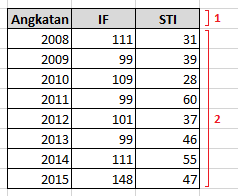
\includegraphics[width=0.3\textwidth]{resources/chapter-3-simple-dataframe.png}
    \caption{Contoh \textit{Data Frame} Sederhana}
	\label{DataFrameSederhana}
\end{figure}

	\subsection{Secara Manual oleh Pengguna}
	Penentuan label dan data dilakukan oleh pengguna secara langsung saat pembuatan tabel. Pengguna sendiri yang menentukan area mana yang merupakan label dan data mana yang dijelaskan oleh label tersebut. Dengan metode manual ini, pengguna dapat menyesuaikan bentuk tabel sesuai keinginan mereka. Metode ini menyerahkan sepenuhnya tanggungjawab keterhubungan sel label dan sel data kepada pengguna.

	\subsection{Secara Otomatis}
	Pencarian label dan data dapat menggunakan algoritma seperti yang telah dijelaskan pada Subbab \ref{metodepencarian}. Mekanisme untuk mengidentifikasi label dan data dapat dilakukan melalui 3 tahapan yakni, \textit{frame finder}, \textit{hierarchy extractor}, dan \textit{tuple builder}. Pada tahap pertama yakni \textit{frame finder} bertujuan untuk mengidentifikasi wilayah nilai (data) dan wilayah atribut (label) yang dapat berupa \textit{left attribute} maupun \textit{top attribute}. Tahap selanjutnya adalah \textit{hierarchy extractor} bertujuan untuk mendapatkan hirarki dari atribut-atribut yang ada sehingga label yang tertulis dapat dicari keterhubungan dan konteksnya terhadap data yang ada. Tahap terakhir adalah \textit{tuple builder} yang mentrasformasikan data dan label tersebut dalam bentuk \textit{tuple} yang dapat diterima oleh basis data relasional.

	\subsection{Perbandingan Metode Penentuan}
    (ini harusnya dibagian perbandingan?)
	Namun, karena algoritma ini hanya optimal jika digunakan pada tabel yang terurut vertikal, maka diperlukan intervensi pengguna untuk menentukan mana tabel yang dimaksud untuk dapat meningkatkan akurasi.

\section{Pengecekan Integritas dan Kesesuaian Data}
Pengecekan integritas dan kesesuaian data dilakukan untuk mengurangi kesalahan masukan yang terjadi dan menyesuaikan tipe yang diterima oleh tabel pada basis data. 

\section{Penyimpanan dan Pemulihan Data}

